\begin{figure}[tb!]
\centering
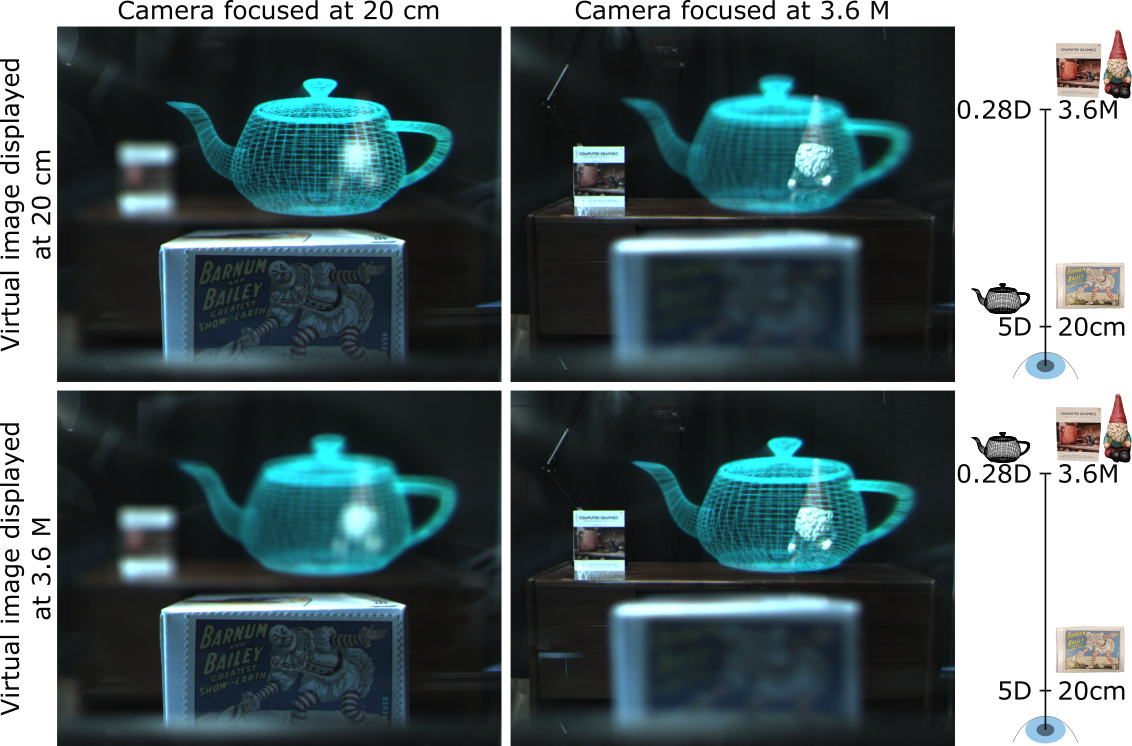
\includegraphics[width=\columnwidth]{images/volumetric/single_plane_images}
\caption[Volumetric NED: Examples of individual depth planes]{View through our near-eye display when only one out of the 280 binary image planes is encoded with a binary image. This figure gives an idea of how each binary image is perceived by an eye or a camera. When all binary images are encoded with appropriate content, a time-integrated color volume occupying a large depth range can be seen (see Figure~\ref{fig:volumetric:results}).}
\label{fig:volumetric:single_plane_images}
\end{figure}

